
%(BEGIN_QUESTION)
% Copyright 2011, Tony R. Kuphaldt, released under the Creative Commons Attribution License (v 1.0)
% This means you may do almost anything with this work of mine, so long as you give me proper credit

Two different level transmitters are used as redundant sensing devices for a critical vessel in a petrochemical refining process where a high level condition is dangerous but a low level condition is safe.  A ``high select'' voting algorithm ignores the lowest-reading transmitter signal.  The reliability rating ($R$) for each transmitter -- describing its probability of faithfully sensing liquid level inside the vessel -- is shown on the diagram:

$$\includegraphics[width=15.5cm]{i00225x01.eps}$$

Determine the {\it MooN} ratings for this redundant transmitter system, from the perspective of {\it dependability} (i.e. the {\it MooN} rating describing its ability to detect a dangerous (high) level condition), as well as from the perspective of {\it security} (i.e. the {\it MooN} rating describing its ability to keep the process running).

\vskip 10pt

MooN (dependability) = \underbar{\hskip 50pt}  \hskip 70pt MooN (security) = \underbar{\hskip 50pt}

\vskip 40pt

Next, calculate the overall reliability that this two-transmitter system will be able to initiate a shutdown if needed, based on the individual reliability ratings given:

\vskip 10pt

$R_{shutoff}$ = \underbar{\hskip 50pt}

\underbar{file i00225}
%(END_QUESTION)





%(BEGIN_ANSWER)

{\it 2 points for each MooN answer, plus 6 points for the reliability calculation}

\vskip 10pt

MooN (dependability) = \underbar{\bf 1oo2}  \hskip 70pt MooN (security) = \underbar{\bf 2oo2}

\vskip 10pt

$R_{shutoff}$ = \underbar{\bf 0.99985}

%(END_ANSWER)





%(BEGIN_NOTES)

{\bf This question is intended for exams only and not worksheets!}

%(END_NOTES)


